\documentclass[a4paper,10pt]{article}

\usepackage{graphicx}
\usepackage{amsfonts}
\usepackage{amssymb}
\usepackage{amsmath}
\usepackage{latexsym}
\usepackage{enumerate}
\usepackage{mdwlist}

%opening
\title{An Exploration of HQSOMS}
\author{Ted Hilk, Joseph Lynch}

\begin{document}

\maketitle

\begin{abstract}

\end{abstract}

\section{Introduction}
\section{Literature Review}
\section{Hypothesis, Plan, and Risks}
\section{System Design and Variables}
HQSOM based networks consist of three basic building blocks: the Self Organizing Map (SOM), the
Recurrent Self Organizing Map (RSOM) and the SOM-RSOM pair.  By composing SOM-RSOM pairs
into larger networks, Hierarchical Quilted Self-Organizing Maps are formed (HQSOM), which can
identify both spatial and temporal clustering in data.  It is important to note that a sinlg
e SOM-RSOM pair is still an HQSOM. The general use case for HQSOMs is to cluster data, and then a
supervised learner will actually make the classification because clusters in of themselves do not
provide a classification.
\subsection{SOM}
The basic SOM computional block can either be trained on data or asked to classify data. The SOM is
made up of a $m$x$n$ matrix that maps inputs of dimension $m$ to outputs of dimension $n$.  For
example a SOM designed to take in 3d vectors and output a 5d vector looks like:

\begin{center}
$
\begin{pmatrix}
.3 & .7 & .1  & .14 & .01\\
.3 & .1 & .01 & .16 & .9\\
.3 & .03 & .8 & .7  & .01
\end{pmatrix}
$
\end{center}
Each column is a map unit, and whichever map unit $\bold{w_b}$ is closest to the input $\bold{x}$
is considered the best-matching unit (BMU).  The measure of closeness is usually simply Euclidean
distance, so:
\begin{equation}
 \bold{w_b} = argmin_{w_i} ||\bold{x} - \bold{w_i}||
\end{equation}
 
During the training stage, input vectors are applied to the input and then an
update rule is applied over the entire map space that shifts map units that are nearest to the
input data towards the input data:
\begin{equation} \label{eq:UPDATE}
 \bold{w_{i}}(t+1) = \bold{w_i}(t) + \gamma h_{ib}(t)(\bold{x}(t)-\bold{w_i}(t))
\end{equation}
where gamma is the rate of learning, $h_{ib}$ is the neighborhood function, and $\bold{w_i}$ is the
map unit being modified.  The neighborhood function is defined as a function that is close to zero
for units far away from the BMU.  Traditionally a gaussian is used:
\begin{equation} \label{eq:GAUSSIAN}
 h_{ib}(t) = exp(\frac{-||I_i-I_b||^2}{\mu(t)\sigma^2})
\end{equation}
where $I_i$ indicates the index of the $i$th unit, $\mu(t)$ is a decreasing function of mean
squared error and $\sigma$ is the learning radius.  A SOM therefore has two parameters that need to
be tuned: the learning rate $\gamma$ and the learning radius $\sigma$. For example, two sample unit
maps after an update with $\bold{x}=(.1,.1,.1), \gamma=.2$ and different sigmas would look like:
\begin{figure}[h]
\begin{center}
$
\begin{pmatrix}
0.26 &  0.7 &  0.1 &  0.14  & 0.01 \\
0.26  & 0.1  & 0.01 & 0.16 & 0.9  \\
0.26  & 0.03 & 0.8  & 0.7  & 0.01
\end{pmatrix}$
\caption{$\sigma$ = 1}
\centering
$\begin{pmatrix}
0.26 &  0.607 &  0.1 &  0.139  & 0.01 \\
0.26  & 0.1  & 0.017 & 0.159 & 0.897  \\
0.26  & 0.041 & 0.748  & 0.687  & 0.01
\end{pmatrix}
$
\caption{$\sigma$ = 100}
\end{center}
\end{figure}

During activation, the SOM can return two types of activation vectors:
\begin{enumerate}
\item Discrete: A vector of the correct dimension with the BMU index set to 1 and all others set
to 0.
\item Continous: A vector $A(t)$ defined as the normalized form of a vector constructed as follows:
\begin{equation}
 A_i = \frac{1}{||\bold{x(t)} - \bold{w_i}||^2}
\end{equation}
\end{enumerate}


\subsection{RSOM}
The Recurrent SOM is an extension of the basic SOM that adds a exponential moving average of
differences between observed inputs and units in the map with time-decay parameter $\alpha$ . At
each update the differences are updated and instead of looking for the BMU in map space, the BMU
index is chosen by finding the minimum magnitude recursive difference. Furthermore, instead of
applying $\bold{x}(t)$ directly to the map, the recursive difference for a particular unit is
applied in each unit's update rule and $\bold{x}(t)$ is used to update the recursive difference
matrix:
\begin{equation}
 \bold{y_i}(t+1) = (1-\alpha)\bold{y_i}(t)+\alpha(\bold{x}(t)-\bold{w_i}(t))
\end{equation}
The update rule becomes:
 \begin{equation} \label{eq:RUPDATE}
 \bold{w_{i}}(t+1) = \bold{w_i}(t) + \gamma h_{ib_r}(t)\bold{y(t)}
\end{equation}
where the neighborhood function is computed using the recursive BMU as the BMU index instead of the
map space BMU.  Tuning of $\alpha$ depends on how responsive one wants the RSOM to be: lower values
of $\alpha$ mean a moving average of inputs dominate (long term memory) and higher values of
$\alpha$ (close to 1) mean that recent inputs dominate (short term memory).
\subsection{SOM-RSOM Pair}
The final computational structure is the SOM-RSOM pair.  Recognizing that SOMs are effective at
identifying spatial clustering, and RSOMs are effective at identifying temporal clustering, but
SOMs do zero temporal clustering and RSOMs have degraded spatial clustering, the SOM-RSOM pair is
intended to get the best effect of both.  First the input data is fed into the SOM to get a spatial
representation, and then this representation is fed into the RSOM to do temporal clustering. 
\section{Implementation Process and Results}
Two implementations of SOMs and RSOMs were written, one being as close as possible
to the reference implementation for reproduceability, and the other having a number of slight
changes to improve convergance.  As is to be expected, the reference paper leaves out a
number of implementation details so this is our best approximation.
\subsection{Reference Implementation of SOM and RSOM Units}
Self-Organizing Maps were implemented via a python class with three main methods: a constructor,
an update method that takes a numpy array representing the input vector as well as the learning
parameters (gamma, sigma, etc...) and modifies the internal state of the SOM accordingly, and a
method to request the activation vector for a given input vector. Internally the SOM map was stored
as a $m$x$n$ numpy array where $n$ is the input vector size and $m$ is the size of the map space. 
During an update call, the Best Matching Map Unit (BMU) for any given input vector was determined
using a linear search for the minimum Euclidean distance and then all map units near to the BMU as
well as the BMU were shifted towards the input according to a Gaussian neighborhood function.  The
standard SOM update rule was used as per equation ($\ref{eq:UPDATE}$).
 
A linear search was prefered due to the high dimensionality of the space <CITATION NEEDED>, and a
Gaussian neighborhood function was chosen for reproduceability.  The activation
method returned either a discrete or a continuous representation of the map's activation to a given
input. The discrete representation is defined as above, and the normal representation is given in
equation ($\ref{eq:EUCMETH}$) where $a_i$ represents the $i$th position in the activation vector,
$\bold{w_b}$ is the BMU, $\bold{x}$ is the input vector, and $\bold{w_i}$ represents the $i$th map
unit.
\begin{equation} \label{eq:EUCMETH}
 a_i = \frac{1}{||\bold{w_i}-\bold{x}||}, \bold{a} = \frac{\bold{a}}{||\bold{a}||}
\end{equation}
\\
Recurrent Self-Organizing Maps were simply a subclass of the SOM that use the modified RSOM update
rule as well as storing the recursive difference matrix as a numpy array.  The time decay parameter
($\alpha$) was passed in at every update call.

\subsection{Basic Design of SOM-RSOM Pair and Other Hierarchical Structures}
Since both SOMs and RSOMs are implemented as Python objects, the SOM-RSOM pair simply consisted of
a SOM object and a RSOM object with an update and activation method that takes in an input vector
$\bold{x}$, feeds it into the SOM to get a transformed activation vector $\bold{y}$ and finally
takes that $\bold{y}$ and feeds it into the RSOM to get the final output which is the BMU of the
RSOM.  The only difference between the SOM-RSOM update and activation methods is that the update
method is calling update internally while the activation method is passing along activation
vectors. In the code this SOM-RSOM pair was refered to as a HQSOM because a single SOM-RSOM pair
does indeed form the simplest HQSOM.

Hierarchies were built at first by hard wiring these HQSOM base units together.  However, in order
to facilitate testing of the audio extension, a framework was designed that allowed for any
arbitrary tree HQSOM taking a linear input.  The first level of the tree reads data from the input,
and passes its activation vector to the next layer, which passes its activation vector to the next
layer, etc ...

\subsection{Replication of First Experiment}
The first experiment presented in the paper was a simple example of 3x3 images with 3
pixel horizontal and vertical lines that have been shifted to all possible positions.  This data
set is small enough to be enumerated, and simple enough in concept to use a single SOM-RSOM pair as
the HQSOM network.  We implemented the network as a single HQSOM that had an input size of 9,
internal SOM map size of 18, and internal RSOM map size of 3.  We mapped the 3x3 image grids
to a linear vector of size 9 by iterating through the image left to right and top to bottom.
The mapping used is shown in Figure $\ref{fig:3TestMapping}$.
\begin{figure}[ht]
\begin{center} 
$\begin{pmatrix}
1 & 2 & 3 \\
4 & 5 & 6 \\
7 & 8 & 9 
\end{pmatrix}
\rightarrow
\begin{pmatrix}
1 & 2 & 3 & 4 & 5 & 6 & 7 & 8 & 9 
\end{pmatrix}
$
\end{center} 
\caption{Experiment 1 Image to Vector Mapping}
\label{fig:3TestMapping}
\end{figure} 

The implementation was shown to be correct by three different tests: performance on non-noisy
data, performance on noisy data, and aggregate performance over many noisy data sets. During
training, the HQSOM is exposed to three blank images, followed by three line images, followed by
three blank images where the three line images alternate between the three horizontal and the three
vertical images. An example training sequence without noise is shown in Figure
$\ref{fig:3TestData}$.
\begin{figure}[ht]
\begin{center} 
 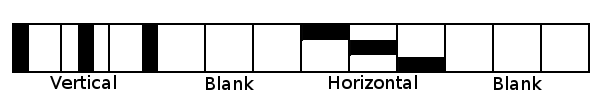
\includegraphics[scale=.3]{./exp1_dataset.png}
 % exp1_dataset.png: 200x200 pixel, 72dpi, 7.05x7.05 cm, bb=0 0 200 200
\end{center} 
\caption{Experiment 1 Training Sequence}
\label{fig:3TestData}
\end{figure} 
Applying the sequence shown in Figure $\ref{fig:3TestData}$ hundreds of times trains the HQSOM and
clusters the weight vectors in the map units of the SOM and RSOM.  Since the blank images are
soley meant to reset the RSOM EMA difference matrix, a method was added to RSOMs and HQSOMs that
allows the difference matrix to be cleared (with a random index selected to have a value of .01 so
that the BMU varies randomly after each reset) and the training steps with blank images were
replaced with a call to this function. After roughly 2500 training samples were shown to the
network, the HQSOM was asked to classify (return the BMU of the top level RSOM) each piece of data
again and as expected all horizontal lines were classified the same, all vertical Lines were
classified the same, and all blank images were classified the same regardless of position.  The
netork had successfully formed an invariant representation of vertical and horizontal lines in a
3x3 field of view.
\\
To test the noise tolerance of the network, gaussian noise with standard deviation .1, .2, .25 and
.3 was applied to the test data, which was then trained on as before and the HQSOM was again asked
to classify samples of noisy vertical and horizontal lines (with different noise from the training
data).  The results are summarized in Table $\ref{fig:3TestResults}$.
 

\subsection{Replication of Second Experiment}

\subsection{Changes to Algorithm and Relative Performance}

and $MSE(\bold{x},\bold{y})$ indicates the mean squared error between vectors $\bold{x}$ and
$\bold{y}$.
\begin{equation} \label{eq:MSEMETH}
 a_i = \frac{MSE(\bold{w_b}, \bold{x})^3}{MSE(\bold{w_i},\bold{x})^3}
\end{equation}
The first method is fairly common in SOM implementations, but the second is intended to downplay the
results of non-matching units, which should theoretically increase orthagonality while preserving
noise tolerance.

\subsection{Extension into Audio}
\subsection{Problems}
\section{Discussion and Conclusions}
\section{References}

\begin{thebibliography}{}
\bibitem{HQSOM} J. W. Miller and P. H. Lommel. \textsc{Biomimetic sensory abstraction using
hierarchical quilted self-organizing maps}. The Charles Stark Draper Laboratory, Inc.
555 Technology Square, Cambridge, MA 02139-3563, USA. 2006.
\end{thebibliography}

\end{document}
